\section{Introduction}
Blockchain technology has revolutionized the way we create trustless and decentralized applications, offering immense composability and the ability to build complex primitives. However, the blockchain landscape is far from homogeneous, with multiple ecosystems that are based on their own consensus protocols and offer varying security and operation features. 

Axelar\footnote{\url{https://axelar.network}} enables interoperability between diverse blockchain ecosystems. Axelar is based on the Cosmos SDK\footnote{\url{https://cosmos.network}} and aims to interlink various blockchain ecosystems, such as Cosmos, Ethereum, Bitcoin, Polygon, and others. Notably, it has been identified as one of only two possible solutions that are sufficiently secure across the stack to be used by the leading decentralized exchange, Uniswap~\cite{uniswap-report}.

Ethereum, in particular, is one of the most widely used blockchains, hosting a multitude of decentralized applications spanning various sectors, including finance, gaming, and governance\cite{wood,buterin}. Therefore, establishing a seamless and secure connection to Ethereum is of paramount importance for Axelar. This proposal focuses on building a trustless connection between Axelar and Ethereum.

\subsection{Current Construction}
Currently, Axelar implements a Tendermint-based delegated proof-of-stake consensus mechanism~\cite{axelar-whitepaper,buchman2019latest}. In particular, validators lock stake in the Axelar chain and receive stake delegations from Axelar users. The top $75$ validators, based on the aggregate (self and delegated) stake, are chosen to participate in Axelar's consensus mechanism.

Axelar adopts a modular architecture to connect with different chains. Each connector module consists of two essential components. The first component verifies source chain data (e.g., Ethereum) into Axelar. The second component generates threshold signatures, which can be verified on the source chain. In this report, we focus exclusively on the former, that is verification of source chain data that are bridged into Axelar.

Currently, connectors utilize an on-chain voting mechanism within Axelar to verify transactions that occur on the source chain. The validators who participate in a connector attestation are called \emph{attestors}. To determine the voting power of an attestor, Axelar employs quadratic voting. Briefly, the voting power of an attestor is the square root of their total stake. This mechanism aims to ensure a fair distribution of influence among attestors, based on their stake. Attestors are required to run a full node of the source chain and have access to the full node's RPC (Remote Procedure Call) interface. This enables them to verify the finalized transactions on the source chain, before voting to bridge them on Axelar.

To bridge data from the source chain to Axelar, a user interacts with an Axelar smart contract on the source chain. Subsequently, the user accesses the connector module on Axelar and initiates a voting poll, which is viewed by attestors. For each poll, an attestor decides whether to vote for or against. To make an informed decision, the attestor queries the source chain's full node RPC and checks if the
transaction under question has been finalized on the source chain. If a poll receives sufficient attestations, it is accepted, otherwise it is rejected.

This voting process forms the basis of verifying the source chain data into Axelar.
Nonetheless, for the connector construction to function securely, both the source chain and Axelar are assumed safe and live. In addition, the (quadratic) voting power distribution among the attestors is assumed to have an honest majority.

\subsection{Problem Statement}
The current construction of Axelar relies on attestors running the full node of
the source chain to verify transactions and vote in an informed manner.
As the Axelar network expands its support for additional chains,
attestors will be required to run an increasing number of full nodes to verify
transactions from these source chains.

However, running a full node, or many, imposes significant costs on
attestors.\footnote{Indicatively, running a full Ethereum node requires $4+$
CPU cores, $16+$ GB RAM, at least $1$ TB SSD, and $25$ Mbps of stable
connection (source:
\url{https://www.quicknode.com/guides/infrastructure/node-setup/ethereum-full-node-vs-archive-node}).}
In order to maintain a diverse and robust ecosystem, comprising a multitude of
participants, it is important to develop cost-effective and efficient
solutions.\footnote{In practice, systems that impose significant costs for running a full node often demonstrate centralization tendencies, where participants tend to rely on
third-party service providers to run and maintain the full nodes on their behalf. Due to economies of scale, a large portion of these networks tends to cluster around a small number of such providers; e.g., at times, $50$\% of Ethereum's transactions ran through one such provider, Infura~\cite{infura}. Therefore, proactively addressing such hazards can lead to a healthier, more diverse and robust ecosystem.}
Such solutions could reduce the entry and maintenance costs for new validators,
also possibly leading to more value being gained for users.

To address this challenge, we propose a construction that enables users and attestors to verify the consensus of the source chain within the Axelar execution layer. This is accomplished through light and super-light client constructions of the source chain.

In this report, we explore several constructions for light and super-light clients tailored specifically for Ethereum. We then propose a construction that best aligns with Axelar's vision and requirements, aiming to drive decentralization, enhance security, and improve scalability. Our construction makes use of Ethereum's sync committee and guarantees bridge safety, assuming at least one Axelar attestor is honest.

\begin{figure}
    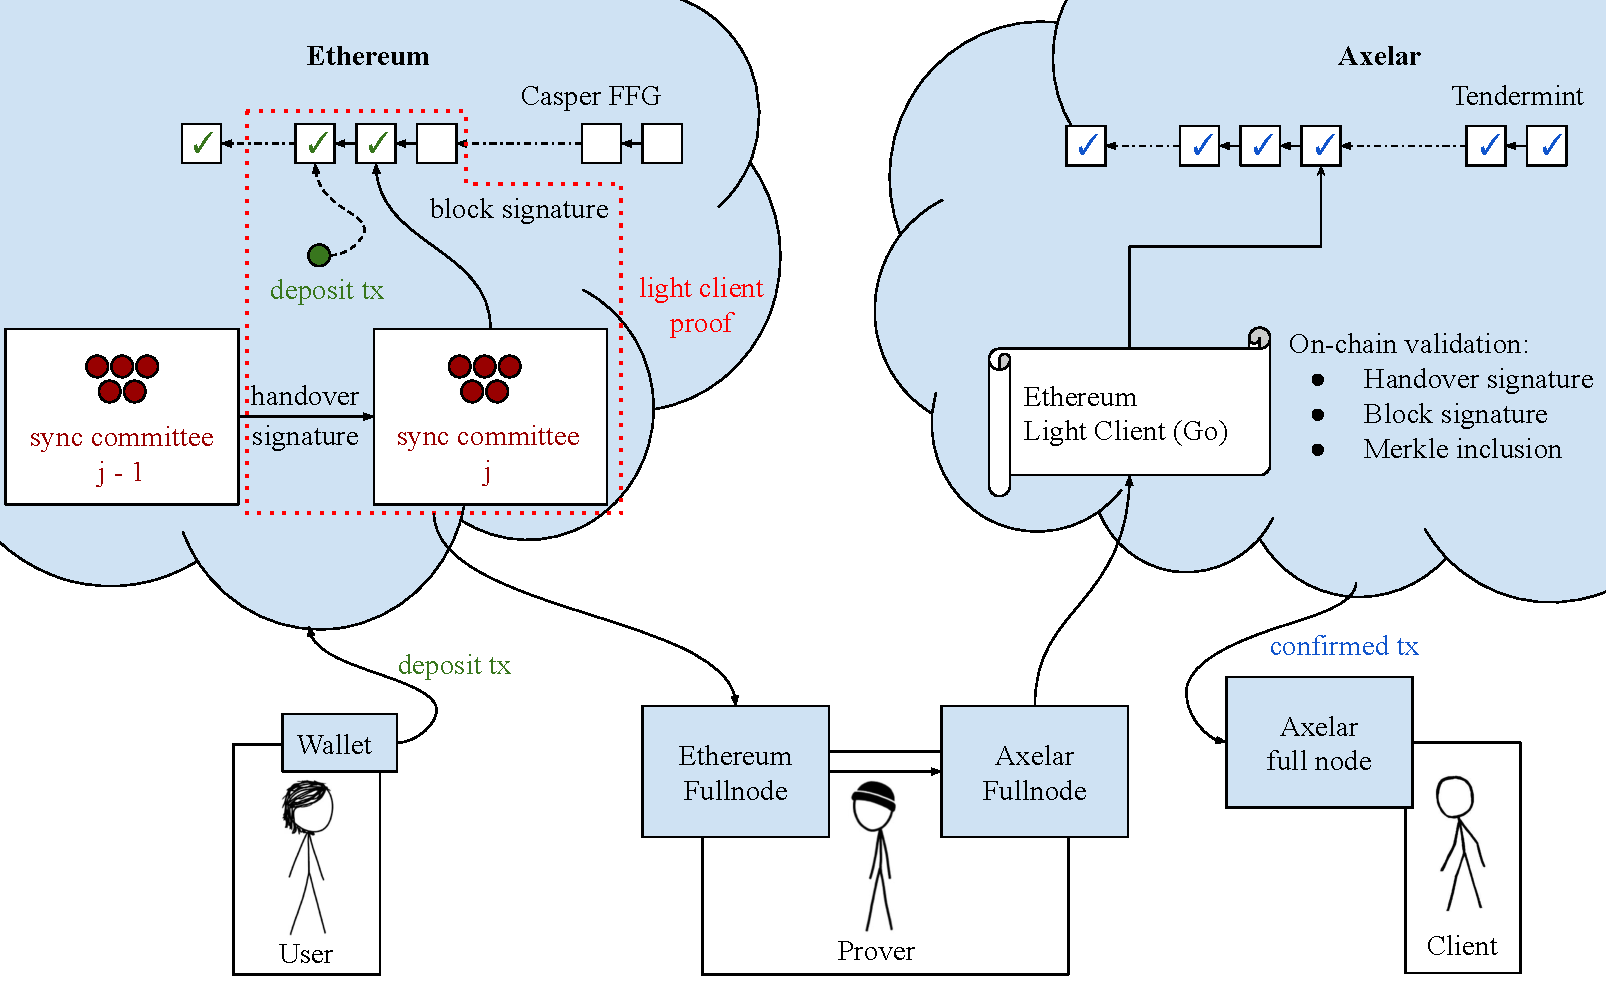
\includegraphics[scale=0.55]{figures/axelar_light_client_architecture.pdf}
    \caption{We recommend implementing an on chain light client using sync committee. The light client will be implemented as a go module that will be deployed on the Axelar network. The light client will be responsible for verifying the handover signatures, block signatures and Merkle inclusion proofs.}
    \label{fig.axelar_light_client_architecture}
\end{figure}


